\begin{figure}[htbp]
  \centering
  \begin{minipage}{.84\textwidth}
  \centering\small
  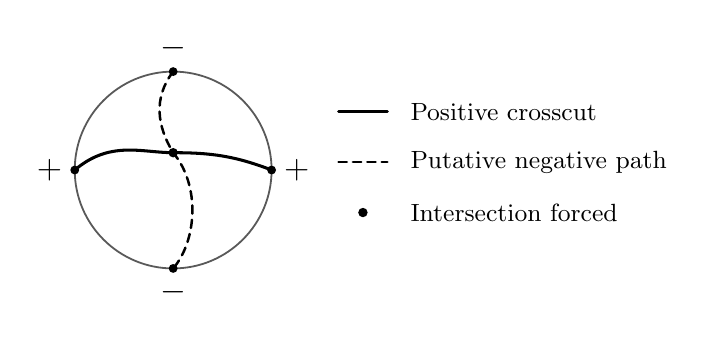
\begin{tikzpicture}[x=1cm,y=1cm,font=\small,
      line cap=round,line join=round]
    \draw[black!65,line width=.65pt] (0,0) circle[radius=1.25];
    \node at (-.67,-.69) {$\D$};

    \draw[line width=1.1pt]
      (-1.25,0) .. controls (-.8,.38) and (-.4,.22) .. (0,.22)
      .. controls (.48,.22) and (.78,.18) .. (1.25,0);

    \draw[line width=.9pt,dash pattern=on 3pt off 2.2pt]
      (0,1.25) .. controls (-.26,.91) and (-.20,.55) .. (0,.22)
      .. controls (.35,-.20) and (.30,-.90) .. (0,-1.25);
    \fill (0,.22) circle[radius=1.7pt];

    \foreach \x/\y in {-1.25/0,1.25/0,0/1.25,0/-1.25}
      \fill (\x,\y) circle[radius=1.6pt];
    \node[font=\large] at (-1.57,0) {$+$};
    \node[font=\large] at (1.57,0) {$+$};
    \node[font=\large] at (0,1.55) {$-$};
    \node[font=\large] at (0,-1.55) {$-$};

    \draw[line width=1.1pt] (2.10,.74) -- (2.72,.74);
    \node[anchor=west] at (2.89,.74) {Positive crosscut};
    \draw[line width=.9pt,dash pattern=on 3pt off 2.2pt]
      (2.10,.10) -- (2.72,.10);
    \node[anchor=west] at (2.89,.10) {Putative negative path};
    \fill (2.41,-.54) circle[radius=1.7pt];
    \node[anchor=west] at (2.89,-.54) {Intersection forced};
  \end{tikzpicture}
  \caption{Connectedness of the positive set gives a crosscut joining the
  $+$ points. It separates the two $-$ points, forcing any negative connecting
  path to meet it. The dashed path illustrates this contradiction; all four
  boundary signs are strict.}
  \label{fig:boundary-signs}
  \end{minipage}
\end{figure}
